%%%%%%%%%%%%%%%%%%%%%%%%%%%%%%%%%%%%%%%%%
% University Assignment Title Page
% LaTeX Template
% Version 1.0 (27/12/12)
%
% This template has been downloaded from:
% http://www.LaTeXTemplates.com
%
% Original author:
% WikiBooks (http://en.wikibooks.org/wiki/LaTeX/Title_Creation)
%
% License:
% CC BY-NC-SA 3.0 (http://creativecommons.org/licenses/by-nc-sa/3.0/)
%
% Instructions for using this template:
% This title page is capable of being compiled as is. This is not useful for
% including it in another document. To do this, you have two options:
%
% 1) Copy/paste everything between \begin{document} and \end{document}
% starting at \begin{titlepage} and paste this into another LaTeX file where you
% want your title page.
% OR
% 2) Remove everything outside the \begin{titlepage} and \end{titlepage} and
% move this file to the same directory as the LaTeX file you wish to add it to.
% Then add \input{./title_page_1.tex} to your LaTeX file where you want your
% title page.
%
%%%%%%%%%%%%%%%%%%%%%%%%%%%%%%%%%%%%%%%%%
%\title{Title page with logo}
%----------------------------------------------------------------------------------------
%	PACKAGES AND OTHER DOCUMENT CONFIGURATIONS
%----------------------------------------------------------------------------------------

\documentclass[12pt]{article}
\usepackage[french]{babel}
\usepackage[utf8x]{inputenc}
\usepackage{amsmath}
\usepackage{graphicx}
\usepackage[colorinlistoftodos]{todonotes}
\usepackage{listings}
\usepackage{float}
\usepackage[justification=centering]{caption}
\usepackage[toc,page]{appendix}
\usepackage{url}
\begin{document}

\begin{titlepage}

\newcommand{\HRule}{\rule{\linewidth}{0.5mm}} % Defines a new command for the horizontal lines, change thickness here

\center % Center everything on the page

%----------------------------------------------------------------------------------------
%	HEADING SECTIONS
%----------------------------------------------------------------------------------------

\textsc{\LARGE SORBONNE UNIVERSITE}\\[1.5cm] % Name of your university/college
\textsc{\Large Projet SAR}\\[0.5cm] % Major heading such as course name
\textsc{\large }\\[0.5cm] % Minor heading such as course title

%----------------------------------------------------------------------------------------
%	TITLE SECTION
%----------------------------------------------------------------------------------------

\HRule \\[0.4cm]
{ \huge \bfseries Ordonnancement de processus avec prise en compte de la synchronisation}\\[0.4cm] % Title of your document
\HRule \\[1.5cm]

%----------------------------------------------------------------------------------------
%	AUTHOR SECTION
%----------------------------------------------------------------------------------------

\begin{minipage}{0.4\textwidth}
\begin{flushleft} \large
\emph{Auteurs:}\\
Pierre-Loup \textsc{Gosse}\\
Salim Toufik \textsc{Nedjam}\\
Aymeric \textsc{Ploton}
\end{flushleft}
\end{minipage}
~
\begin{minipage}{0.4\textwidth}
\begin{flushright} \large
\emph{Encadrants:} \\
Redha \textsc{Gouicem}\\
Julien \textsc{Sopena}
\end{flushright}
\end{minipage}\\[2cm]

% If you don't want a supervisor, uncomment the two lines below and remove the section above
%\Large \emph{Author:}\\
%John \textsc{Smith}\\[3cm] % Your name

%----------------------------------------------------------------------------------------
%	DATE SECTION
%----------------------------------------------------------------------------------------

{\large \today}\\[2cm] % Date, change the \today to a set date if you want to be precise

%----------------------------------------------------------------------------------------
%	LOGO SECTION
%----------------------------------------------------------------------------------------


\includegraphics[scale=0.35]{include/logo_sorbonne.png}  % Include a department/university logo - this will require the graphicx package
\hspace{1cm}

\includegraphics[scale=0.15]{include/logo_lip6.png}\\ % Include a department/university logo - this will require the graphicx package

%----------------------------------------------------------------------------------------

\vfill % Fill the rest of the page with whitespace

\end{titlepage}

%-------------------------------------------------------------------------------
% BODY
%-------------------------------------------------------------------------------

%\tableofcontents

\section*{Introduction}
L'une des tâches les plus importantes qu'un OS doit faire est de faciliter le
multi-tasking.
C'est l'ordonnanceur qui s'occupe de cette tâche critique.

L'ordonnanceur à pour but premier de performer cette fonction le plus
efficacement possible en utilisant le moins de ressources, et en respectant les
trois principes qui sont Safety, Liveness et Fairness.
\\

Les objectifs de notre projet ont donc été les suivants: optimiser les
décisions de l'ordonnanceur pour apporter une élection plus favorable aux
processus détenant un verrou.
\\

Nous verrons tout d'abord dans ce rapport les différents aspects de la Glibc
qui permet de gérer la synchronisation. 

Ensuite, nous aborderons les différents points qui font le lien entre la Glibc
et le kernel. 

Enfin, nous présenterons notre approche d'ordonnancement des processus.

\section*{Problématique}

Le problème se présente quand plusieurs processus souhaitent accéder à une même
ressource critique. En effet, considérons un processus A (de haute priorité) qui
se met à attendre un processus B (moins propriétaire), ce dernier peut se faire déscheduler
par un processus C dont la priorité est: 

Pri(A) $>$ Pri(C) $>$ Pri(B), cela va retarder
l'élection du processus A car le processus B qui détient la ressource 
évoluera lentement. 

Il est donc important de faire passer en priorité dans les 
élections le processus détenant cette section tout en respectant la prévalence
des autres processus indépendants pour respecter la sémantique du CFS 
(Completly Fair scheduler).
\\

Pour résoudre ce problème il a fallu dans un premier temps permettre au
kernel de connaître l'identité du processus propriétaire du verrou.
Ensuite le scheduler devait utiliser cette information et agir en conséquence.
\\

\section*{Glibc et mutex}
La Glibc offre un panel de fonctionnalités. 
Celle des verrous (mutex) nous intéresse particulièrement: elle permet 
d'abstraire aux programmeurs l'utilisation complexe des verrous côté kernel.
\\

Il existe 4 types de mutex proposés à l'utilisateur :
\begin{enumerate}
	\item TIMED: type par défaut, prend le verrou de manière bloquante.
	\item RECURSIVE: ne tente pas de prendre le verrou si celui-ci est
	déjà détenu par le processus courant.
	\item ADAPTIVE: correspond à la méthode de prise de verrou 'trylock',
	au bout d'un certain nombre d'échec la prise de verrou se fait
	bloquante.
	\item ERRORCHECK: prend le verrou ne manière brutale en évitant
	simplement les problèmes de contention.
\end{enumerate}
Le choix du type de mutex se fait lors de l'initialisation du verrou.
\\
On peut combiner ces 4 types externes avec des types internes qui permettent de
modifier le comportement du verrou jusqu'au kernel:
\newpage
\begin{enumerate}
	\item ROBUST: type par défaut, si le propriétaire du verrou meurt sans
	le relâcher la prochaine demande à se verrou sera accepté sans appel
	système.
	\item PI (Priority Inheritance): la priorité du processus détenant le
	verrou est augmenté à la plus grande priorité parmi les processus
	bloqués sur le verrou.
	\item PP (Priority Protect): le processus à sa priorité déterminé par
	sa configuration grâce à 'priority ceiling'.
\end{enumerate}
Les types ROBUST et PI insère le \textit{pid} du propriétaire du verrou
directement dans la valeur du verrou. Ainsi lors des appels systèmes le kernel
peut connaître le \textit{pid} du propriétaire du verrou avec une simple
opération de flag sur la valeur passée.
\\

En tenant compte de ces éléments on peut donc en déduire que la modification 
de la partie Glibc n'est pas nécessaire. En effet le \textit{pid} du 
propriétaire du verrou étant déjà communiqué il nous suffit de le récupérer 
côté kernel. Ainsi cela permet à notre futur solution de ne pas dépendre de 
modification ou de décoration d'une fonctionnalité de la Glibc
\newpage
\section*{Kernel et futex}
La Glibc communique avec le kernel à travers des appels systèmes, elle fournit 
en paramètre l'adresse virtuelle de l'espace utilisateur qui contient la 
valeur du lock.
\\

Cette dernière est convertie par une fonction de hashage en clé unique qui 
identifie un futex donné, elle est ensuite utilisée dans un bucket pour lister
tous les processus en attente d'un futex donnés.
\\

Pour permettre au kernel de bien suivre l'évolution du possesseur du lock, Il a
fallu créer une structure \verb|futex_state| pour gérer l'état d'un futex, elle se
présente comme ci-dessous:
\begin{lstlisting}
	struct futex_state {
		struct list_head list;
		struct rt_mutex mutex;
		struct task_struct *owner;
		atomic_t refcount;
		union futex_key *key;
	};

\end{lstlisting}
\\

Pour que les informations reflètent l'état exact du futex
à un instant \textit{t}, il faut que la structure \verb|futex_state| soit mise à jour
à chaque changement de l'état du futex. Ainsi, chaque processus avant de 
s'endormir sur un futex indique dans un champ de sa structure task l'adresse de 
la structure \verb|futex_state| du futex sur lequel il va s'endormir.
\\

Par conséquent chaque processus après avoir manipulé le futex 
devra chercher dans une liste chaînée la structure \verb|futex_state| associée au 
futex et la mettre à jour avec la valeur courante du lock. Ainsi à tout moment le kernel peut savoir sur quel futex un processus prioritaire et endormi 
et quel est le processus qui détient ce futex.

\section*{Scheduler}

Depuis sa version 2.6.23 le kernel utilise le Completely Fair Scheduler (CFS), il est aujourd'hui le scheduler par défaut. Une bonne compréhension de son fonctionnement a donc été nécessaire pour envisager des modifications.
\\

Le CFS fonctionne sur un système d'arbre: le \verb|rbtree|. L'arbre permet de créer une timeline sur les futurs tâches à exécuter. 
Il est composé de \verb|sched_entity|, ces entités regroupe une ou plusieurs tâches, permettant ainsi de faire des lots d'exécution. Chaque entité a un poids (\verb|load|), et un compteur du temps d'exécution virtuel passé dans le CPU (\verb|vruntime|). Ces deux données permettent au scheduler d'organiser son arbre d'exécution: les entités sont réparties par ordre croissant à partir de leur \verb|vruntime|, de gauche à droite. Ainsi, à gauche de l'arbre se trouve l'entité avec la valeur \verb|vruntime| la plus faible, c'est cette entité qui sera choisi lors de l'élection par le scheduler.
\\

L'équité est le maître mot du scheduler CFS. Son but est de partager le temps CPU entre chaque processus en fonctions des autres tâches exécutable. Pour ce faire, le CFS utilise un technique de découpage temporelle: le \verb|timeslice|. Chaque entité se voit attribuer un poids (\verb|load|) qui est calculé dépendamment des autres tâches courantes. Ainsi, une entité avec une priorité plus élevé aura une poids plus important. Prenons un exemple, deux tâches de même priorité doivent se partager un temps d'utilisation CPU de 10 ms, appelé \verb|target time|. Les deux tâches ont donc le même poids, le CFS attribuera aux tâches une \verb|timeslice| de 5 ms d'utilisation CPU. Si nous prenons maintenant deux tâches où leur différence de priorité est de 5, soit par exemple 10 et 15, avec une \verb|target time| de 20 ms, le poids diffère et la tâche la moins prioritaire se verra attribuer 1/3 du \verb|target time| soit une \verb|timeslice| de 5 ms contre 15 ms pour l'autre tâche.
\\

Le cœur du fonctionnement du CFS se repose sur son horloge virtuelle : la \verb|virtual clock|. Cette horloge permet au scheduler de mesurer un temps d'exécution virtuel sur le CPU pour chaque entité. Cette valeur est stocké dans la variable \verb|vruntime|. L'entité élu se voit mettre à jour ses statistiques fréquemment, c'est ici que sa valeur \verb|vruntime| est mise à jour. Le principe est le suivant : à chaque fois qu'une entité s'exécute dans le CPU le timestamp est sauvegardé dans la variable \verb|exec_start|, à chaque mise à jour de \verb|vruntime| la différence entre le timestamp actuelle et \verb|exec_start| est calculé dans la variable \verb|delta_exec|, la valeur de cette dernière sera divisé par le poids de l'entité puis ajouté au \verb|vruntime|. Ainsi, plus la priorité est élevé plus la valeur ajouté au \verb|vruntime| sera faible et par conséquent l'entité avancera lentement vers la droite de l'arbre (Figure \ref{fig:sched}).
\\

\begin{figure}[h!]
	\centering
	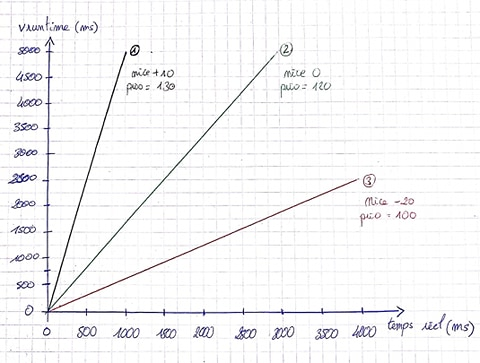
\includegraphics[scale=0.6]{schema_sched.jpg}
	\caption{Relation entre le vruntime et le temps réel en fonction de la priorité}
	\label{fig:sched}
\end{figure}
\\

De part ces faits nous pouvons en déduire que pour prioriser une entité, représentant une tâche détenant un verrou, nous pouvons influencer sur son \verb|vruntime| pour la garder à gauche de l'arbre et assurer une réélection rapide. Cependant cette solution peut présenter plusieurs problèmes. Le code du scheduler reste complexe et une modification aussi importante peut facilement causer des problèmes dans des cas d'exécution non prévu. Étant donné que la valeur \verb|vruntime| se base sur la priorité de l'entité nous avons décidé de ne pas toucher au code du scheduler et d'accélérer les tâches en modifiants habilement leur priorité.











%\include{p3}

%\include{conclusion}

%\include{annexe}
\clearpage

%\bibliographystyle{plain}
%\bibliography{bibliography}

\end{document}
